\chapter*{Проектирование системы}
\addcontentsline{toc}{chapter}{Проектирование системы}

\section*{Концептуальный дизайн}
\addcontentsline{toc}{section}{Концептуальный дизайн}

\subsection*{Концептуальная модель системы в нотации IDEF0}
\addcontentsline{toc}{subsection}{Концептуальная модель системы в нотации IDEF0}

Для создания функциональной модели портала, отражающей его основные функции и потоки информации наиболее наглядно использовать нотацию IDEF0. На рисунке \ref{img:idef0-0} приведена концептуальная модель системы. На рисунке \ref{img:idef0-1} представлена декомпозиция функциональной модели системы.

\includeimage
{idef0-0} % Имя файла без расширения (файл должен быть расположен в директории inc/img/)
{f} % Обтекание (без обтекания)
{H} % Положение рисунка (см. figure из пакета float)
{\textwidth} % Ширина рисунка
{Концептуальная модель в нотации IDEF0} % Подпись рисунка

\includeimage
{idef0-1} % Имя файла без расширения (файл должен быть расположен в директории inc/img/)
{f} % Обтекание (без обтекания)
{H} % Положение рисунка (см. figure из пакета float)
{\textwidth} % Ширина рисунка
{Детализированная концептуальная модель в нотации IDEF0} % Подпись рисунка


\subsection*{Сценарии функционирования системы}
\addcontentsline{toc}{subsection}{Сценарии функционирования системы}

Для детальной разработки портала используется унифицированный язык моделирования UML. В системе выделены 2 роли: администратор и пользователь (авторизованный и неавторизованный). На рисунках \ref{img:use-case-admin}-\ref{img:use-case-user} представлены диаграммы прецедентов для выделенных ролей и описаны сценарии функционирования наиболее значимых прецедентов.

\includeimage
{use-case-user} % Имя файла без расширения (файл должен быть расположен в директории inc/img/)
{f} % Обтекание (без обтекания)
{H} % Положение рисунка (см. figure из пакета float)
{\textwidth} % Ширина рисунка
{Диаграмма прецедентов для роли <<пользователь>>} % Подпись рисунка

\includeimage
{use-case-admin} % Имя файла без расширения (файл должен быть расположен в директории inc/img/)
{f} % Обтекание (без обтекания)
{H} % Положение рисунка (см. figure из пакета float)
{\textwidth / 3} % Ширина рисунка
{Диаграмма прецедентов для роли <<администратор>>} % Подпись рисунка

\subsubsection*{Регистрация пользователя}
\begin{enumerate}
    \item Пользователь переходит на страницу входа с помощью кнопки <<войти>>, либо автоматически перенаправляется на соответствующую страницу при попытке совершения действий, которые невозможно совершить без регистрации (например, покупка или возврат билетов). 
    \item Пользователь нажимает на кнопку <<зарегистрироваться>> и перенаправляется на страницу регистрации, где вводит различные наборы полей. Валидация входных данных осуществляется <<на лету>> на стороне пользователя. При отправке данных на фронтенд, он тоже производит валидацию.
    \item Пользователь нажимает кнопку «Регистрация» и перенаправляется на главную страницу портала.
\end{enumerate}

\subsubsection*{Авторизация на портале клиента или мастера}
\begin{enumerate}
    \item Пользователь переходит на страницу входа с помощью кнопки <<войти>>, либо автоматически перенаправляется на соответствующую страницу при попытке совершения действий, которые невозможно совершить без регистрации (например, покупка или возврат билетов). 
    \item Вводит учётные данные, нажимает кнопку <<войти>>.
    \item Пользователь даёт согласие на использование его данных. Если пользователь не дает согласия, то он перенаправляется на страницу с ошибкой.
    \item Пользователь перенаправляется на главную страницу портала.
\end{enumerate} 

\subsubsection*{Просмотр доступных для покупки билетов}
Сценарий доступен как для авторизованного, так и для неавторизованного пользователя.
\begin{enumerate}
    \item Пользователь задаёт параметры поиска авиабилета (город отправления, город назначения, дату поездки) и нажимает кнопку <<найти>>.
    \item На экране появляется список доступных билетов с детальной информацией о билете (цена, время вылета).
\end{enumerate}

\subsubsection*{Покупка билета}
Сценарий доступен только для авторизованного пользователя.
\begin{enumerate}
    \item Пользователь задаёт параметры поиска авиабилета (город отправления, город назначения, дату поездки) и нажимает кнопку <<найти>>.
    \item На экране появляется список доступных билетов с детальной информацией о билете (цена, время вылета).
    \item Пользователь выбирает билет, переходит на страницу с детальной информацией о билете и нажимает кнопку <<купить>>.
    \item Пользователю предлагается выбрать: начислить баллы за покупаемый билет или списать баллы с бонусного счёта для уменьшения цены билета.
    \item С бонусным счётом производится операция в соответствии с выбранном на предыдущем шаге действием пользователя.
\end{enumerate}

\subsubsection*{Возврат билета}
Сценарий доступен только для авторизованного пользователя.
\begin{enumerate}
    \item Пользователь выбирает кнопку <<личный кабинет>> на главной странице портала.
    \item В разделе <<купленные билеты>> пользователь выбирает билет, который хочет вернуть, и нажимает соответствующую кнопку.
    \item С бонусным счётом производятся дейтсвия, обратные к совершённым при покупке билета. При этом остаток на бонусном счёт не может быть отрицательным.
\end{enumerate}

\subsubsection*{Просмотр операций с бонусным счётом}
Сценарий доступен только для авторизованного пользователя.
\begin{enumerate}
    \item Пользователь выбирает кнопку <<личный кабинет>> на главной странице портала.
    \item Пользователь открывает раздел <<история операций с бонусным счётом>> и перенаправляется на страницу с историей.
\end{enumerate}

\subsubsection*{Получение статистики}
\begin{enumerate}
    \item Пользователь с ролью <<администратор>> нажимает на кнопку <<посмотреть историю запросов>> и перенаправляется на соответствующую страницу.
	\item Пользователь с ролью <<администратор>> нажимает на кнопку <<Получить статистику>>.
	\item Пользователь перенаправляется на страницу просмотра статистики о запросах.
\end{enumerate}

\subsubsection*{Спецификация сценария покупки билета}
Нормальный ход сценария.
\begin{table}[!h]
	\begin{center}
		\caption{\label{spec_buy_ticket}Спецификация покупки билета} 
		\footnotesize
		\begin{tabular}{|l|l|}
			\hline	
   \multicolumn{1}{|c|}{\begin{tabular}[c]{@{}c@{}}Действия актера\end{tabular}} & 
    \multicolumn{1}{c|}{\begin{tabular}[c]{@{}c@{}} Отклик системы\end{tabular}}  \\
\hline выбор билета из списка доступных & открытие страницы с \\
& подробной информацией о билете \\
\hline запрос покупки билета & успешная проверка авторизации и запрос подтверждения операции \\
\hline подтверждение операции & осуществление покупки \\
\hline
	\end{tabular}
	\end{center}
\end{table}

Альтернативный ход сценария.
\begin{table}[!h]
	\begin{center}
		\caption{\label{spec_buy_ticket}Спецификация покупки билета} 
		\footnotesize
		\begin{tabular}{|l|l|}
			\hline	
   \multicolumn{1}{|c|}{\begin{tabular}[c]{@{}c@{}}Действия актера\end{tabular}} & 
    \multicolumn{1}{c|}{\begin{tabular}[c]{@{}c@{}} Отклик системы\end{tabular}}  \\
\hline выбор билета из списка доступных & открытие страницы с \\
& подробной информацией о билете \\
\hline запрос покупки билета & успешная проверка авторизации и запрос подтверждения операции \\
\hline отклонение операции & покупка не осуществляется \\
\hline
	\end{tabular}
	\end{center}
\end{table}
\newpage
Альтернативный ход сценария.
\begin{table}[!h]
	\begin{center}
		\caption{\label{spec_buy_ticket}Спецификация покупки билета} 
		\footnotesize
		\begin{tabular}{|l|l|}
			\hline	
   \multicolumn{1}{|c|}{\begin{tabular}[c]{@{}c@{}}Действия актера\end{tabular}} & 
    \multicolumn{1}{c|}{\begin{tabular}[c]{@{}c@{}} Отклик системы\end{tabular}}  \\
\hline выбор билета из списка доступных & открытие страницы с \\
& подробной информацией о билете \\
\hline запрос покупки билета & неуспешная проверка авторизации,  \\
& перенаправление на страницу ввода учётных данных \\
\hline
 ввод учётных данных  & успешная проверка учётных данных,  \\
 & запрос подтверждения операции \\
\hline подтверждение операции & осуществление покупки\\
\hline
	\end{tabular}
	\end{center}
\end{table}
\section*{Логический дизайн}
\addcontentsline{toc}{section}{Логический дизайн}

\subsection*{Диаграммы классов}
\addcontentsline{toc}{subsection}{Диаграммы классов}

Иерархии классов для разработки серверных приложений представлены в виде диаграммы классов:
\begin{itemize}
    \item сервиса рейсов --  на рисунке \ref{img:flights_uml};
    \item сервиса билетов --  на рисунке \ref{img:ticket_uml};
    \item сервиса сессий и пользователей --  на рисунке \ref{img:person_uml};
    \item сервиса программы лояльности --  на рисунке \ref{img:bonus_uml};
    \item сервиса-координатора --  на рисунке \ref{img:gateway_uml};
    \item сервиса оплаты --  на рисунке \ref{img:bank_uml};
    \item сервиса статистики --  на рисунке \ref{img:stat_uml}.
\end{itemize}


\includeimage
{flights_uml} % Имя файла без расширения (файл должен быть расположен в директории inc/img/)
{f} % Обтекание (без обтекания)
{H} % Положение рисунка (см. figure из пакета float)
{\textwidth} % Ширина рисунка
{Диаграмма классов сервиса рейсов} % Подпись рисунка

\includeimage
{ticket_uml} % Имя файла без расширения (файл должен быть расположен в директории inc/img/)
{f} % Обтекание (без обтекания)
{H} % Положение рисунка (см. figure из пакета float)
{\textwidth} % Ширина рисунка
{Диаграмма классов сервиса билетов} % Подпись рисунка


\includeimage
{person_uml} % Имя файла без расширения (файл должен быть расположен в директории inc/img/)
{f} % Обтекание (без обтекания)
{H} % Положение рисунка (см. figure из пакета float)
{\textwidth} % Ширина рисунка
{Диаграмма классов сервиса сессий и пользователей} % Подпись рисунка


\includeimage
{bonus_uml} % Имя файла без расширения (файл должен быть расположен в директории inc/img/)
{f} % Обтекание (без обтекания)
{H} % Положение рисунка (см. figure из пакета float)
{\textwidth} % Ширина рисунка
{Диаграмма классов сервиса программы лояльности} % Подпись рисунка


\includeimage
{gateway_uml} % Имя файла без расширения (файл должен быть расположен в директории inc/img/)
{f} % Обтекание (без обтекания)
{H} % Положение рисунка (см. figure из пакета float)
{\textwidth / 2} % Ширина рисунка
{Диаграмма классов сервиса-координатора} % Подпись рисунка


\includeimage
{bank_uml} % Имя файла без расширения (файл должен быть расположен в директории inc/img/)
{f} % Обтекание (без обтекания)
{H} % Положение рисунка (см. figure из пакета float)
{\textwidth / 2} % Ширина рисунка
{Диаграмма классов сервиса оплаты} % Подпись рисунка


\includeimage
{stat_uml} % Имя файла без расширения (файл должен быть расположен в директории inc/img/)
{f} % Обтекание (без обтекания)
{H} % Положение рисунка (см. figure из пакета float)
{\textwidth / 2} % Ширина рисунка
{Диаграмма классов сервиса статистики} % Подпись рисунка
\newpage
\subsubsection{Описание классов сервисов}

Сервисы рейсов, билетов, программы лояльности и сессий и пользователей спроектированы похожим образом. Они имеют:
\begin{itemize}
    \item слой доступа к данным, реализованный с помощью паттерна <<Репозиторий>> для абстракции хранения, а также паттерна <<пул объектов>> для эффективного использования активных подключений к базе данных;
    \item слой логики работы сервиса;
    \item слой интерфейса -- слой связи с другими сервисами с помощью http-запросов.
\end{itemize}

Так как сервисы спроектированы одинаково, часть классов совпадают. Опишем их:
\begin{itemize}
    \item IDAFacade -- абстрактный интерфейс слоя доступа к данным; PGDAFacade -- реализация этого абстрактного интерфейса для работы с данными, хранящимися под управлением СУБД Postgres;
    \item IDAFactory -- абстрактный интерфейс фабрики объектов, относящихся к библиотеке работы с данными (интерфейс спроектирован в соответствии с паттерном <<фабрика объектов>>); PGDAFactory -- реализация этого абстрактного интерфейса для работы с данными, хранящимися под управлением СУБД Postgres;
    \item PGConnection -- пул активных подлключений к базе данных, спроектированный в соответствии с паттерном <<пул объектов>>;
    \item IBLFacade -- абстрактный интерфейс слоя логики; BLFacade -- реализация этого абстрактного интерфейса;
    \item IServer -- абстрактный интерфейс серверного приложения, предоставляющего интерфейс, описанный HTTPController; Server -- реализация этого интерфейса.
    \item HTTPController -- класс, описывающий набор  HTTP-методов, которые доступны на сервисе. Фактически занимается распаковкой данных, пришедших по сети, заполнением необходимых структур этими данными и вызовом функций, реализующих логику работы методов. Также занимается подготовкой результирующих данных к отправке по сети после выполнения запроса. 
\end{itemize}

Кроме того, каждый сервис имеет собственные классы. Опишем их.

\subsubsection{Описание классов сервиса рейсов}

\begin{itemize}
    \item Flight -- класс, описывающий рейс, имеет поля:
    \begin{itemize}
        \item дата и время рейса;
        \item цена рейса;
        \item номер рейса;
        \item аэропорты вылета и прилёта;
        \item города вылета и прилёта.
    \end{itemize}
    \item IFlightRepository -- абстрактный интерфейс для работы с данными рейсов (интерфейс спроектирован в соответствии с паттерном <<репозиторий>>). PGFlightRepository -- реализация этого абстрактного интерфейса для работы с данными, хранящимися под управлением СУБД Postgres.
\end{itemize}

\subsubsection{Описание классов сервиса билетов}

\begin{itemize}
    \item Ticket -- класс, описывающий билет, имеет поля:
    \begin{itemize}
        \item номер билета;
        \item цена билета;
        \item номер рейса;
        \item статус (оплачен или отменён);
        \item идентификатор билета;
        \item владелец билета.
    \end{itemize}
    \item ITicketRepository -- абстрактный интерфейс для работы с данными билетов (интерфейс спроектирован в соответствии с паттерном <<репозиторий>>). PGTicketRepository -- реализация этого абстрактного интерфейса для работы с данными, хранящимися под управлением СУБД Postgres.
\end{itemize}

\subsubsection{Описание классов сервиса сессий и пользователей}

\begin{itemize}
    \item User -- класс, описывающий пользователя, имеет поля:
    \begin{itemize}
        \item идентификатор пользователя;
        \item логин пользователя;
        \item роль пользователя;
        \item возраст пользователя;
        \item пароль пользователя (в виде хэша).
    \end{itemize}
    \item Session -- класс, описывающий сессию пользователя, является JWT-token-ом;
    \item Credentials -- класс, который хранит логин и пароль пользователя.
    \item IUserRepository -- абстрактный интерфейс для работы с данными пользователей и сессий (интерфейс спроектирован в соответствии с паттерном <<репозиторий>>). PGUserRepository -- реализация этого абстрактного интерфейса для работы с данными, хранящимися под управлением СУБД Postgres.
\end{itemize}

\subsubsection{Описание классов сервиса программы лояльности}

\begin{itemize}
    \item BuyRequest -- класс, описывающий запрос на покупку билета, имеет поля:
    \begin{itemize}
        \item решение пользователя о списании или о начислении бонусов;
        \item цена билета;
        \item номер билета;
        \item имя пользователя.
    \end{itemize}
    \item BuyResponse -- класс, описывающий ответ на покупку билета, имеет поля:
    \begin{itemize}
        \item баланс счёта программы лояльности после покупки билета;
        \item количество денег, списанное за счёт бонусов;
        \item количество денег, списанное за счёт средств пользователя;
        \item статус счёта лояльности (золотой, серебряный, бронзовый) после покупки.
    \end{itemize}
    \item BalanceResponse -- класс, описывающий ответ на запрос информации о бонусном счёта и истории операций бонусного счёта, имеет поля:
    \begin{itemize}
        \item баланс счёта программы лояльности;
        \item статус счёта лояльности (золотой, серебряный, бронзовый);
        \item история операций (каждая запись содержит: абсолютное значение изменения баланса, дату операции, типа операции -- списание или начисление, идентификатор билета).
    \end{itemize}
    \item IBonusRepository -- абстрактный интерфейс для работы с данными программы лояльности (интерфейс спроектирован в соответствии с паттерном <<репозиторий>>). PGBonusRepository -- реализация этого абстрактного интерфейса для работы с данными, хранящимися под управлением СУБД Postgres.
\end{itemize}

\subsubsection{Описание классов сервиса-координатора}

\begin{itemize}
    \item HTTPController -- класс, описывающий набор  HTTP-методов, которые доступны на сервисе. Фактически предасвляет собой весь программный интерфейс системы. В своей работе для обслуживания приходящих запросов сервис использует интерфейсы сервисов программы лояльности (BonusService), рейсов (FlightService) и билетов (TicketService). Кроме того, сервис перенаправляет статистику запросов в очередь Kafka с помощью интерфейса KafkaStatistcsService.
    \item Server -- реализация серверного приложения, предоставляющего интерфейс, описанный HTTPController.
\end{itemize}

\subsubsection{Описание классов сервиса оплаты}

\begin{itemize}
    \item HTTPController -- класс, описывающий набор  HTTP-методов, которые доступны на сервисе (покупка и возврат билетов). В своей работе для обслуживания приходящих запросов сервис использует сервисы банка для выполнения транзакций со счётом пользователя.
    \item Server -- реализация серверного приложения, предоставляющего интерфейс, описанный HTTPController.
\end{itemize}

\subsubsection{Описание классов сервиса статистики}
\begin{itemize}
    \item HTTPController -- класс, описывающий набор  HTTP-методов, которые доступны на сервисе (просмотр истории запросов к системе и метрики, рассчитанные на основе этой истории). В своей работе для обслуживания приходящих запросов сервис использует очередь Kafka.
    \item Server -- реализация серверного приложения, предоставляющего интерфейс, описанный HTTPController.
\end{itemize}

\subsection*{Диаграмма деятельности}
\addcontentsline{toc}{subsection}{Диаграмма деятельности}

На рисунке \ref{img:dpd} изображена диаграмма деятельности при покупке билета. 
\includeimage
{dpd} % Имя файла без расширения (файл должен быть расположен в директории inc/img/)
{f} % Обтекание (без обтекания)
{H} % Положение рисунка (см. figure из пакета float)
{0.85\textwidth} % Ширина рисунка
{Диаграмма деятельности при покупке билета} % Подпись рисунка

\newpage
\section*{Высокоуровневый дизайн пользовательского интерфейса}
\addcontentsline{toc}{section}{Высокоуровневый дизайн пользовательского интерфейса}

Пользовательский интерфейс в разрабатываемой системе представляет собой Web-интерфейс, доступ к которому осуществляется через браузер (тонкий клиент).

Страница портала состоит из <<шапки>> (верхней части страницы, в которой находится логотип и верхнее меню со ссылками на основные разделы портала), основной части и <<футера>> (нижней части страницы, в которой обычно размещают ссылки на редко посещаемые, но необходимые, страницы, например, страницы с пользовательским соглашением).

Обобщенно структуру страниц портала можно представить следующим образом:
\begin{itemize}
    \item страница с обучением для пользователя;
    \item главная страница с поиском авиабилетов;
    \item страница подробной информацией о билете и кнопкой покупки;
    \item личный кабинет пользователя (информация о пользователе с возможностью ее изменить);
    \item страница с купленными билетами (с возможностью вернуть еще не использованные билеты);
    \item страница программы лояльности (история операций бонусного счета, остаток на бонусном счёте);
    \item страница входа;
    \item страница регистрации;
    \item страница со статистикой запросов в приложении (доступно администраторам);
    \item о нас (гарантия, способы оплаты, контакты).
\end{itemize}

Ниже приведены основные формы портала. 
\newpage


\includeimage
{mpi_intro} % Имя файла без расширения (файл должен быть расположен в директории inc/img/)
{f} % Обтекание (без обтекания)
{H} % Положение рисунка (см. figure из пакета float)
{\textwidth} % Ширина рисунка
{Форма обучения пользователя} % Подпись рисунка



\begin{figure}[h!]
  \centering
  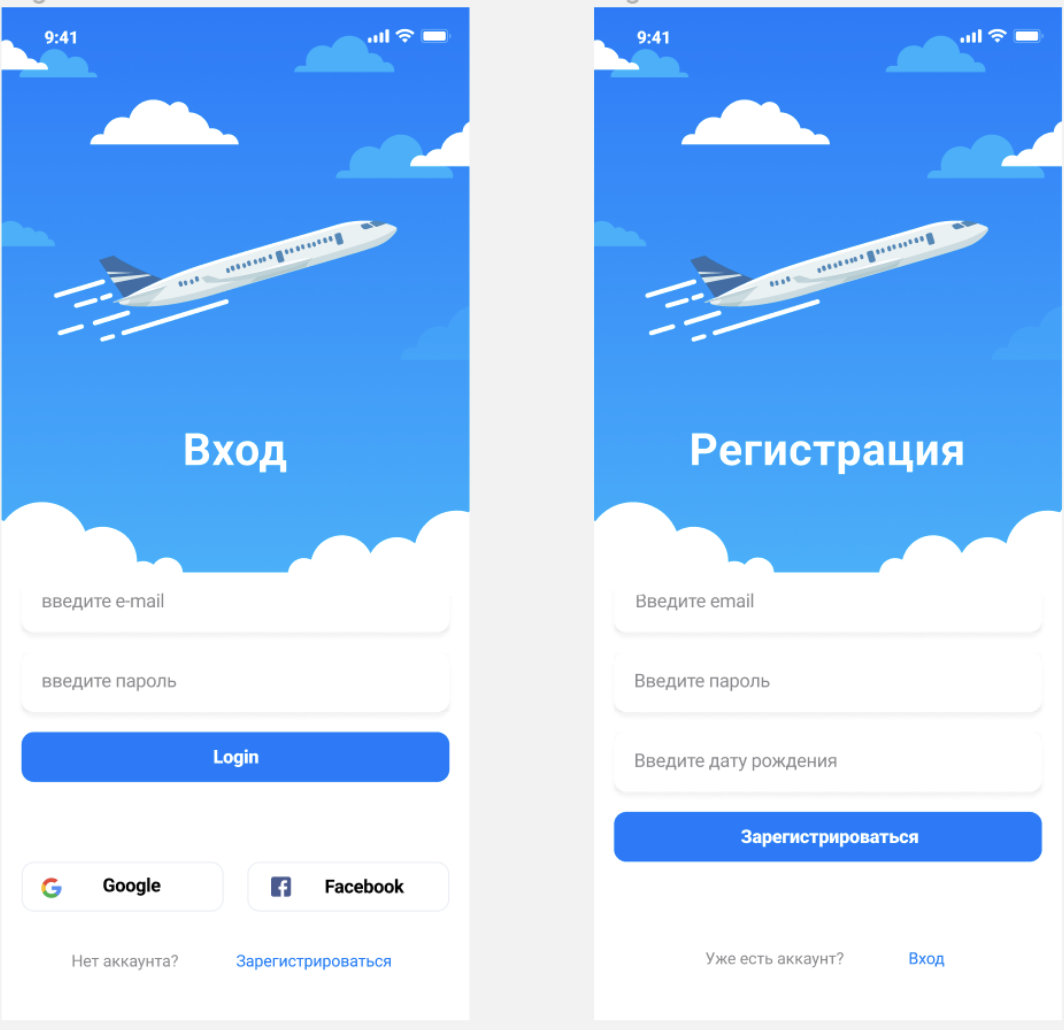
\includegraphics[scale = 0.6]{mpi/inc/img/mpi_login.png}
  \caption{Форма входа и регистрации пользователя}
  \label{fig:scheme}
\end{figure}


\includeimage
{mpi_flights} % Имя файла без расширения (файл должен быть расположен в директории inc/img/)
{f} % Обтекание (без обтекания)
{H} % Положение рисунка (см. figure из пакета float)
{\textwidth} % Ширина рисунка
{Формы с поиском авиабилетов и покупкой билета} % Подпись рисунка


\begin{figure}[h!]
  \centering
  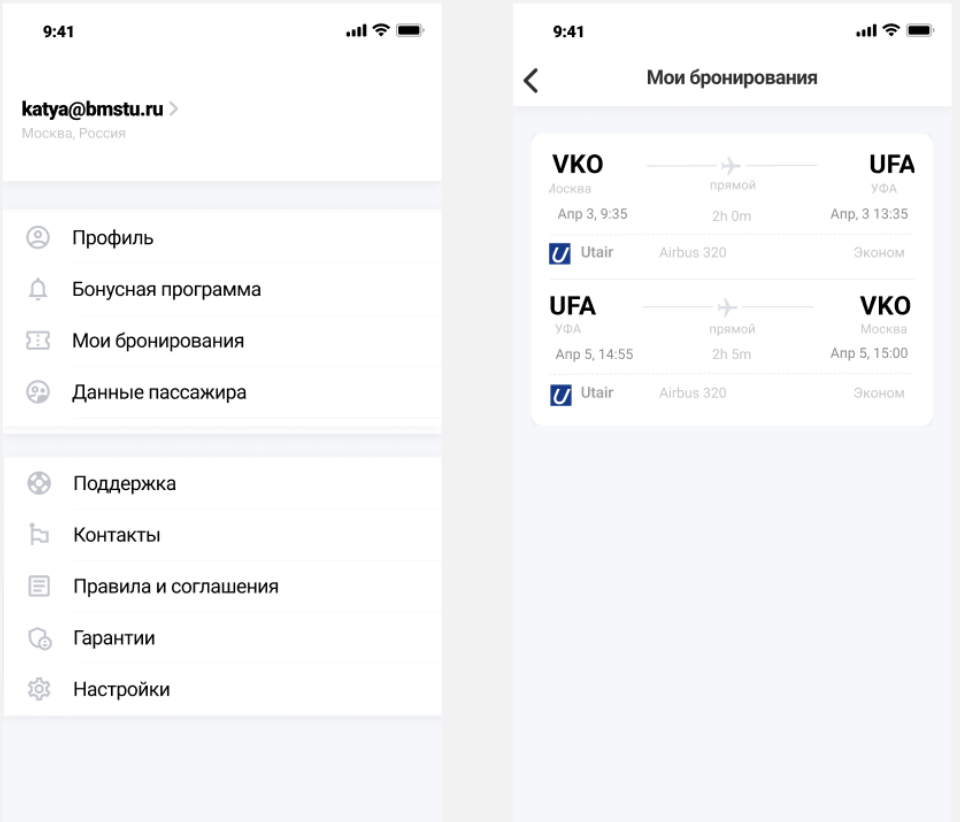
\includegraphics[scale = 0.8]{mpi/inc/img/mpi_account.png}
  \caption{Формы с аккаунтом пользователя и бронированиями}
  \label{fig:scheme}
\end{figure}


\section*{Физический дизайн}
\addcontentsline{toc}{section}{Физический дизайн}

\subsection*{Выбор системы развертывания компонентов распределенной системы}
\addcontentsline{toc}{subsection}{Выбор системы развертывания компонентов распределенной системы}

Согласно требованиям технического задания, разрабатываемая система должна быть распределенной. Характерной особенностью распределенных систем является высокое многообразие используемых технологий. Особенно непростая ситуация возникает, когда разные компоненты системы используют разные версии одной и той же библиотеки. Для того чтобы компоненты не конфликтовали друг с другом, необходимо ввести требование изолированности. В этом случае приходится использовать отдельные серверы, что может быть экономически нецелесообразно, либо использовать контейнеризацию. 

Контейнеризация -- это методология разработки и управления приложениями, которая позволяет упаковывать приложение и все его зависимости в изолированный контейнер (образ изолируемой части системы, содержащий приложение со всеми его зависимостям). Контейнеры обеспечивают среду выполнения для приложения, которая полностью отделена от других контейнеров и основной системы. Это облегчает развертывание, масштабирование и управление приложениями, а также обеспечивает надежность и безопасность при работе в различных средах. 

В качестве платформы для автоматизации развертывания, масштабирования и управления контейнеризированными приложениями на серверах было решено использовать Kubernetes. Такое решение было принято в результате следующего сравнительного анализа.

Существует несколько аналогов Kubernetes, которые также предоставляют возможности для управления контейнеризированными приложениями:
\begin{enumerate}
    \item Docker Swarm -- это оркестратор контейнеров, разработанный Docker, который позволяет управлять кластером Docker-хостов и запускать контейнеры в них. Он более прост в использовании по сравнению с Kubernetes, но может быть менее мощным в некоторых аспектах.
    \item Apache Mesos -- это распределенная система управления ресурсами, которая также поддерживает запуск контейнеров. Он предоставляет более общий подход к управлению ресурсами и приложениями, чем Kubernetes.
    \item Amazon ECS (Elastic Container Service) -- это управляемый сервис от Amazon Web Services для запуска и управления контейнерами на инфраструктуре AWS. Он предлагает простой способ запуска и масштабирования контейнеров без необходимости управления инфраструктурой.
\end{enumerate}

Достоинства Kubernetes по сравнению с аналогами:
\begin{itemize}
    \item Мощные возможности оркестрации: Kubernetes предоставляет широкий спектр возможностей для управления и автоматизации развертывания приложений в контейнерах.
    \item Большое сообщество и экосистема: Kubernetes имеет активное сообщество разработчиков и широкий выбор инструментов и плагинов для расширения его функциональности.
    \item Поддержка различных облачных и локальных сред: Kubernetes поддерживает различные облачные провайдеры и может быть развернут как локально, так и в облаке.
\end{itemize}

\subsection*{Выбор операционной системы}
\addcontentsline{toc}{subsection}{Выбор операционной системы}
Согласно требованиям технического задания, разрабатываемый портал должен обладать высокой доступностью, работать на типичных архитектурах ЭВМ (Intel x86, Intel x64), а так же быть экономически недорогим для сопровождения. Таким образом, можно сформулировать следующие требования к операционной системе:
\begin{itemize}
    \item Распространенность. На рынке труда должно быть много специалистов, способных администрировать распределенную систему, работающую под управлением выбранной операционной системы.
    \item Надежность. Операционная система должна широко использоваться в стабильных проектах, таких как Mail.Ru, Vk.com, Google.com. Эти компании обеспечивают высокую работоспособность своих сервисов, и на их опыт можно положиться.
    \item Наличие требуемого программного обеспечения. Выбор операционной системы недолжен ограничивать разработчиков в выборе программного обеспечения, библиотек.
    \item Цена.
\end{itemize}

Под данные требования лучше всего подходит ОС Ubuntu. Ubuntu -- это дистрибутив, использующий ядро Linux. Как и все дистрибутивы Linux, Ubuntu является ОС с открытым исходным кодом, бесплатным для использования. 

\subsection*{Выбор СУБД}
\addcontentsline{toc}{subsection}{Выбор СУБД}
В качестве СУБД была выбрана PostgreSQL, так как она наилучшим образом подходит под требования разрабатываемой системы:
\begin{itemize}
    \item Масштабируемость: PostgreSQL поддерживает горизонтальное масштабирование, что позволяет распределить данные и запросы между несколькими узлами базы данных. Это особенно полезно в географически распределенных системах, где данные и пользователи могут быть разбросаны по разным регионам.
    \item Географическая репликация: PostgreSQL предоставляет возможность настройки репликации данных между различными узлами базы данных, расположенными в разных географических зонах. Это позволяет обеспечить отказоустойчивость и более быстрый доступ к данным для пользователей из разных частей мира.
    \item Гибкость и функциональность: PostgreSQL обладает широким набором функций и возможностей, что делает его подходящим для различных типов приложений и использования в распределенной среде. Он поддерживает сложные запросы, транзакции, хранимые процедуры и многое другое.
    \item Надежность и отказоустойчивость: PostgreSQL известен своей надежностью и стабильностью работы. В распределенной географической системе это особенно важно, поскольку он способен обеспечить сохранность данных и доступность даже при сбоях в отдельных узлах.
\end{itemize}

\subsection*{Выбор языка разработки и фреймворков компонент портала}
Проанализируем техническое задание на разработку портала. Исходя из приведенных требований к системе, можно выявить требования к языку программирования:
\begin{itemize}
    \item Совместимость с выбранными ранее технологиями. Выбранный язык должен уметь взаимодействовать с ОС Linux, СУБД PostgreSQL.
    \item Производительность: C++ является компилируемым языком программирования, что позволяет создавать быстродействующие приложения. Он обладает низким уровнем абстракции, что позволяет разработчику более тонко управлять ресурсами и оптимизировать производительность программы.
    \item Расширяемость: C++ обладает возможностью использовать объектно-ориентированный подход к программированию, что делает его удобным для создания сложных и масштабируемых систем.
\end{itemize}

Выбор oatpp в качестве фреймворка для разработки программного обеспечения также имеет свои преимущества и может быть обоснован следующими аспектами:
\begin{itemize}
    \item Высокая производительность: oatpp является легковесным и быстрым фреймворком, который спроектирован для обеспечения высокой производительности приложений. Он оптимизирован для работы с сетевыми запросами и обработки данных, что позволяет создавать эффективные веб-сервисы.
    \item Поддержка многопоточности: oatpp предоставляет удобные инструменты для работы с многопоточностью, что позволяет создавать параллельные и распределенные приложения. Это особенно важно для систем, где требуется обработка большого количества запросов одновременно.
    \item RESTful API: oatpp поддерживает разработку RESTful API, что делает его удобным выбором для создания веб-сервисов и API. Он предоставляет инструменты для удобной маршрутизации запросов, валидации данных и других задач, связанных с разработкой веб-приложений.
    \item Модульность и расширяемость: oatpp построен на основе модульной архитектуры, что позволяет легко добавлять новый функционал и расширять возможности фреймворка. Это делает его гибким инструментом для разработки различных типов приложений.
\end{itemize} 

\subsection*{Обеспечение надежности портала}
\addcontentsline{toc}{subsection}{Обеспечение надежности портала}

В данной системе для обеспечения надежности функционирования СУБД будет применяться репликация и шардинг. Для обеспечения надежности данных СУБД необходимо разработать скрипт для автоматического создания резервной копий базы данных по расписанию.

Для фронтенда и бекендов целесообразно применить зеркалирование. Это обеспечит отказоустойчивость системы: в случае сбоя любого из ее узлов запросы на чтение данных будут выполняться. 
